\documentclass[journal]{IEEEtran}

\usepackage[T1]{fontenc}
\usepackage{amsmath,amssymb,amsfonts}
\usepackage{graphicx}
\usepackage{booktabs}
\usepackage{array}
\usepackage{algorithm}
\usepackage[noend]{algpseudocode}
\usepackage{cite}
\usepackage{url}
\usepackage{textcomp}
\usepackage{placeins}
\usepackage{fancyhdr}

% --- page numbers at the bottom right; running head kept at the top left ---
\setlength{\headheight}{12pt}
\pagestyle{fancy}
\fancyhf{}
\renewcommand{\headrulewidth}{0pt}
\renewcommand{\footrulewidth}{0pt}
\fancyhead[L]{\scriptsize\leftmark}
\fancyfoot[R]{\thepage}
\fancypagestyle{plain}{%           % title page: IEEEtran would put the number in the head
  \fancyhf{}%
  \renewcommand{\headrulewidth}{0pt}%
  \renewcommand{\footrulewidth}{0pt}%
  \fancyhead[L]{\scriptsize\leftmark}%
  \fancyfoot[R]{\thepage}%
}

% --- give floats more room so tables/figures do not spill into later sections ---
\renewcommand{\topfraction}{0.92}
\renewcommand{\bottomfraction}{0.85}
\renewcommand{\textfraction}{0.07}
\renewcommand{\floatpagefraction}{0.72}
\setcounter{topnumber}{3}
\setcounter{bottomnumber}{2}
\setcounter{totalnumber}{5}
% double-column floats: allow them to share a page with text instead of being pushed
% onto sparse float pages
\renewcommand{\dbltopfraction}{0.92}
\renewcommand{\dblfloatpagefraction}{0.80}
\setcounter{dbltopnumber}{3}

% --- measured quantities (Section U of the companion notebook); single source of truth ---
\newcommand{\PLNCH}{11\,700}          % active channels per context
\newcommand{\PLMASEL}{$126$~ms}       % MaxActive threshold sweep, decision only
\newcommand{\PLMASTEP}{$141$~ms}      % MaxActive full link update, fixed beam
\newcommand{\PLMASTEPBW}{$144$~ms}    % MaxActive full link update, + beamwidth search
\newcommand{\PLPREDUS}{$1.3$~ms}      % surrogate: feature extraction + inference

\begin{document}

\title{Machine-Learning Surrogates for MaxActive Channel Selection in\\
Terahertz Drone-to-Drone Communications}

\author{Korhan Erdo\u{g}du, \"Ozg\"ur G\"urb\"uz, and Akhtar Saeed%
\thanks{Manuscript prepared July 2026. The authors are with the Faculty of
Engineering and Natural Sciences, Sabanc\i{} University, Istanbul, Turkey (e-mail:
korhan.erdogdu@sabanciuniv.edu; ogurbuz@sabanciuniv.edu; akhtar.saeed@sabanciuniv.edu).
K.~Erdo\u{g}du is the main contributor; \"O.~G\"urb\"uz and A.~Saeed supervised the
project. \emph{(Corresponding author: Korhan Erdo\u{g}du.)}}}

\markboth{IEEE Transactions on Aerospace and Electronic Systems (Correspondence)}%
{Erdo\u{g}du \MakeLowercase{\textit{et al.}}: ML Surrogates for MaxActive Channel Selection in THz Drone Links}

\maketitle
\thispagestyle{plain}   % override IEEEtran's title-page style so p.1 is numbered at the foot

\begin{abstract}
Terahertz (THz) drone-to-drone links promise multi-gigabit capacity, but channel quality
is highly sensitive to distance, molecular absorption, and mobility-induced beam
misalignment. The MaxActive algorithm returns the capacity-maximizing channel subset, yet
it is search-based and must be re-executed at every geometry update, which makes its
per-update cost the bottleneck for an airborne platform. This correspondence asks whether
machine learning can supply a low-complexity surrogate for that search. From a
physics-consistent THz model we reproduce the MaxActive capacity for four mobility
patterns and benchmark eighteen regressors under a leakage-safe nested cross-validation
protocol. A Gaussian process reproduces the reference with a cross-validated $R^2$ of
$0.99$, whereas single decision trees, plain boosting, and unregularized linear regression
fail and overshoot the physical bound most severely. A dueling double deep $Q$-network,
formulated as a single-step contextual bandit, instead learns the \emph{selection} itself,
so it cannot exceed the reference and matches it to within $0.1\%$ on average. The learned
decision costs \PLPREDUS{} against \PLMASEL{} for the search it replaces, from a stored
model of a few kilobytes, and the accompanying complexity analysis shows the most accurate
models to be the most expensive, with tree ensembles the better compromise at scale.
\end{abstract}

\begin{IEEEkeywords}
Beam misalignment, channel selection, complexity, contextual bandit, cross-validation,
deep reinforcement learning, drone communications, Gaussian process, machine learning,
surrogate model, terahertz.
\end{IEEEkeywords}

\section{Introduction: Problem and Proposed Solution}
\IEEEPARstart{T}{erahertz} (THz) bands ($0.1$--$10$~THz) offer the enormous contiguous
bandwidth required by future aerial backbones and dense drone swarms, where fiber is
impractical and lower bands are congested. Propagation in this regime, however, is
uniquely hostile: it is dominated by frequency-selective molecular absorption, whose
spectral lines carve the usable band into narrow transmission windows, and by a
spreading loss that grows with the square of both distance and frequency
\cite{jornet}. The useful capacity of a drone-to-drone link therefore depends on a
tightly coupled set of physical and system quantities: the three-dimensional distance,
the antenna gain and beamwidth, the beam alignment, the per-channel molecular
absorption and thermal re-radiation noise, the selected channel subset, and the
power-allocation policy. Aerial mobility continuously perturbs the geometry, so beams
that are aligned at one instant become misaligned at the next, collapsing the
achievable capacity by many orders of magnitude, and making the online choice of which
channels to activate a first-order determinant of link performance.

The reference solution to the spectrum-selection part of this problem is
\emph{MaxActive}, a threshold-sweep algorithm that returns the channel subset
maximizing capacity for the current channel state. MaxActive is accurate and is treated
throughout this work as the ground-truth reference, but it is search-based: it
repeatedly evaluates capacity while sweeping a signal-to-noise ratio (SNR) threshold,
and it must be re-executed whenever the geometry changes.

\emph{Why a surrogate is needed.} That search cost is not incidental. The sweep
re-evaluates capacity across every channel of a wide THz band, so a single selection takes
tens of milliseconds on a desktop CPU. Aerial mobility perturbs the geometry
continuously, so the search must run at the geometry-update rate, on an embedded processor
that is simultaneously flying the aircraft. A learned model returns the same decision
roughly two orders of magnitude faster and moves the training burden offline;
Section~\ref{sec:complexity} reports the underlying complexity and measurements. The
research question is therefore whether a learned \emph{surrogate} can reproduce the
MaxActive decision directly from the channel state at a fraction of the cost.

We pursue two complementary answers: \emph{supervised regressors} that predict the
MaxActive capacity value from a compact set of physical features, and a \emph{dueling
double deep $Q$-network} (D3QN) that learns the \emph{selection decision} itself and
evaluates the true capacity of its choice, so that it respects the reference bound by
construction. The contributions are fourfold.
(i) A physics-consistent reproduction of the MaxActive water-filling (WF) and equal-power
(EP) capacity curves for \emph{four} mobility patterns, including mobility over elevation
and measured windy-hover acceleration traces. All are regenerated from the reference model
rather than digitized from published figures, which gives a reusable ground truth for
learning.
(ii) The first systematic benchmark, to our knowledge, of eighteen regressors spanning six
model families as surrogates for THz channel selection, under a leakage-safe nested
cross-validation protocol suited to this small-sample, wide-dynamic-range regime.
(iii) The contrast between learning the capacity \emph{value} and learning the selection
\emph{decision}; the latter matches MaxActive to within $0.1\%$ on average and cannot
violate the physical bound.
(iv) A deployment-oriented complexity analysis that combines asymptotic cost with
\emph{measured} execution time and memory footprint.
These four threads --- ground truth, surrogate benchmark, value-versus-decision, and
deployability --- are followed throughout.

\section{Proposed ML Models versus MaxActive}
\label{sec:proposed}
Two facts organize the entire study. First, MaxActive returns the capacity-maximizing
channel subset within its threshold-search family (Section~\ref{sec:background}-B), so
within the adopted system model it upper bounds any surrogate trained to imitate it. When
predictions are compared against that reference we therefore evaluate them at the ceiling,
\begin{equation}
\hat{C}_{\text{clip}}=\min\!\big(\hat{C},\,C_{\text{MaxActive}}\big).
\label{eq:clip}
\end{equation}
Equation~\eqref{eq:clip} requires $C_{\text{MaxActive}}$ --- precisely what a deployed
surrogate does not have, for if it were available online there would be no reason to learn
a surrogate at all. \emph{The clip is therefore an offline evaluation and visualization
device only}. It is applied when plotting against the known reference, so that a displayed
curve never claims an unattainable capacity. It is \emph{not} part of the online
prediction path: at deployment the surrogate emits $\hat{C}$ (or, for the D3QN, a
selection) with no access to the reference. Accordingly, every quantitative error in
Section~\ref{sec:perf} is computed from raw, unclipped predictions, and the ceiling
violations the clip would hide are reported explicitly in Table~\ref{tab:cv}. Second, the
capacity spans roughly nine orders of magnitude across the scenarios
(Table~\ref{tab:maxactive}), so the models are trained on $\log_{10}$ capacity, the
natural scale on which a THz capacity curve is smooth.

The models fall into two categories. Supervised regressors reproduce the capacity
\emph{value}: cheap at inference, but able to exceed the reference bound, which is what
makes unclipped reporting necessary. The D3QN reproduces the selection \emph{decision};
since it evaluates the real capacity of the channels it selects, it is bounded above by
MaxActive automatically and needs no clip at all. Fig.~\ref{fig:allmethods} overlays all
methods on the MaxActive curves for the aligned and diagonal scenarios.

\begin{figure*}[!tp]
\centering
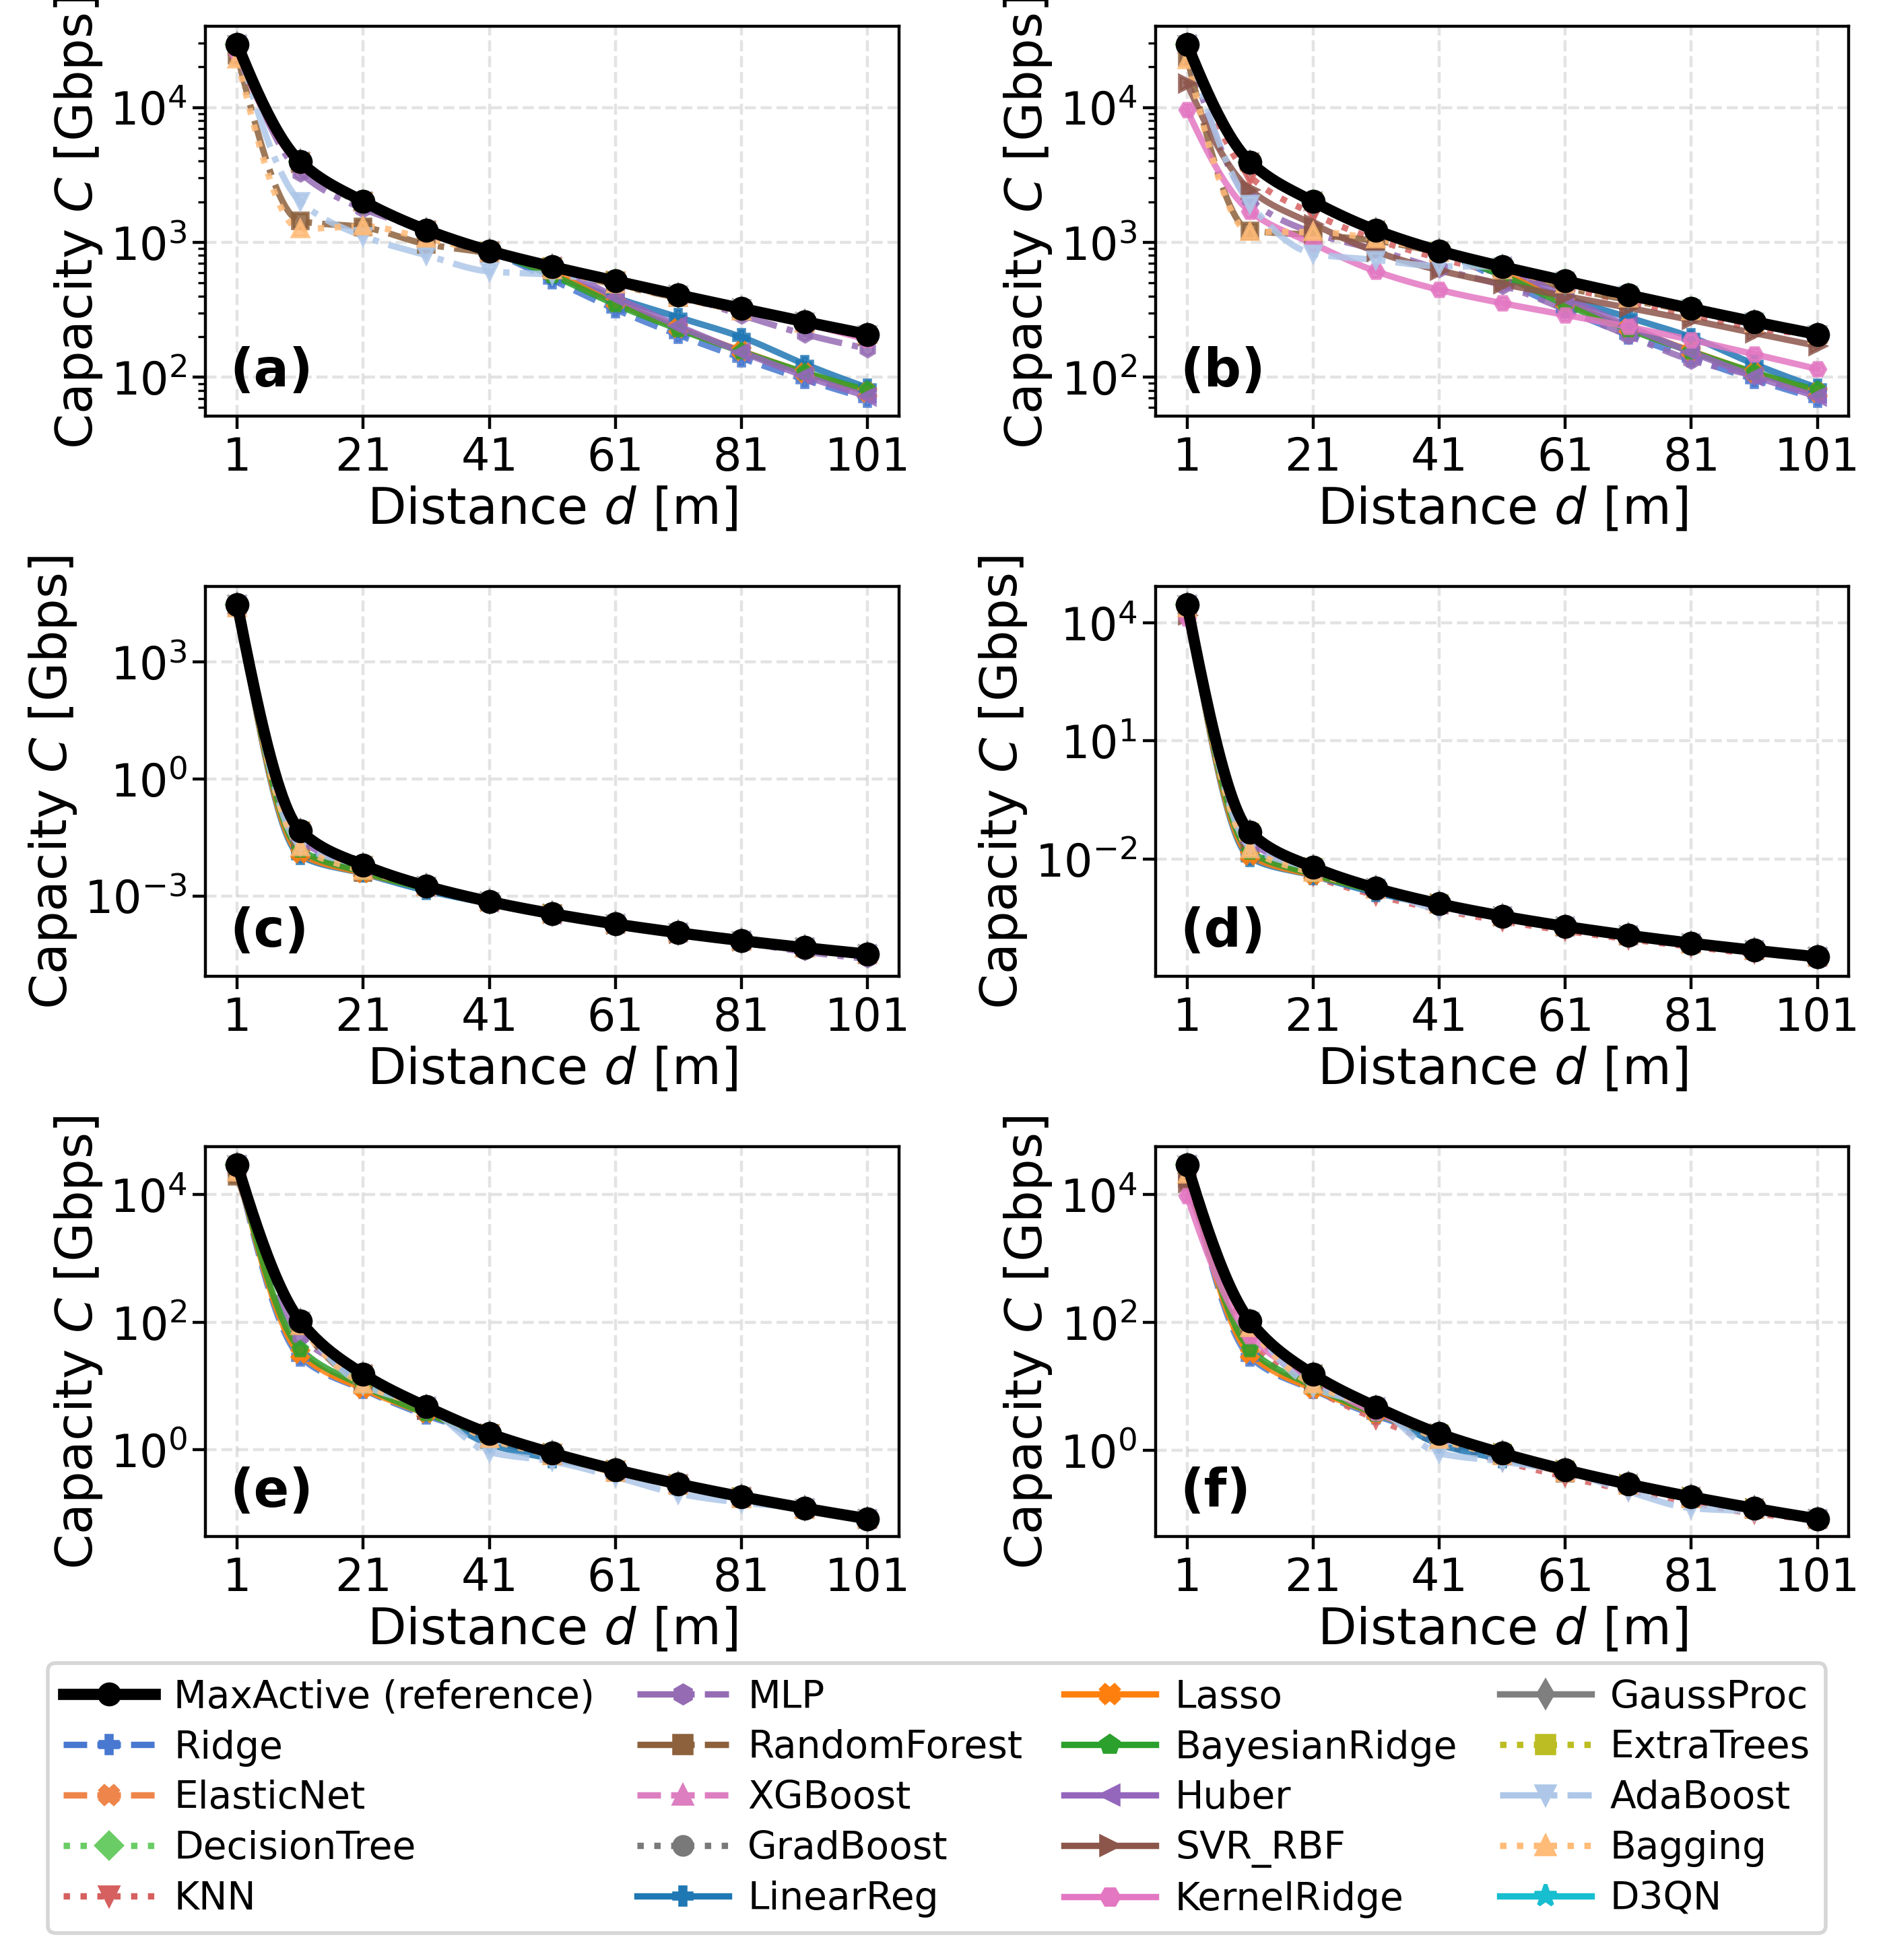
\includegraphics[width=0.76\textwidth]{all_methods_comparison.png}
\caption{All methods versus MaxActive. Rows are mobility scenarios and columns are power
allocations: (a),(b) aligned; (c),(d) misaligned diagonal without beamwidth adjustment;
(e),(f) misaligned diagonal with beamwidth adjustment; WF in (a),(c),(e) and EP in
(b),(d),(f). Curves are models fit on all $33$ samples, evaluated at the MaxActive
ceiling \eqref{eq:clip} for display only, and smoothed by monotone (PCHIP)
interpolation; markers denote the true computed points. The D3QN policy is shown on the
EP column. Note the logarithmic capacity axis.}
\label{fig:allmethods}
\end{figure*}

\section{Alternative ML Solutions}
\label{sec:zoo}
To avoid committing to a single hypothesis class a priori, we evaluate eighteen
regressors spanning six families, all named in Table~\ref{tab:cv}: linear/regularized
(LinearReg, Ridge, Lasso, ElasticNet, BayesianRidge), robust linear (Huber),
kernel/probabilistic (SVR-RBF, KernelRidge, GaussProc), instance-based ($k$-NN), neural
(MLP), and tree ensembles (RandomForest, ExtraTrees, Bagging, AdaBoost, GradBoost,
XGBoost) with a single DecisionTree as contrast. The rationale is physical. In the $\log$
domain the capacity is approximately affine in log-distance and gain, so the
regularized-linear models are the natural baselines. The kernel and probabilistic models
(SVR-RBF, kernel ridge, and a Gaussian process with a squared-exponential-plus-noise
kernel \cite{rasmussen}) capture smooth nonlinear structure, $k$-NN interpolates locally,
and the MLP is a flexible approximator. The tree ensembles are strong tabular learners,
but their piecewise-constant form cannot extrapolate the wide dynamic range. All models
use scikit-learn \cite{sklearn} except XGBoost \cite{xgboost}.

\emph{Why these eighteen suffice.} The set is representative rather than exhaustive: it
covers every hypothesis class standard for small-sample tabular regression and, within
each, spans the inductive biases that could plausibly differ on this target. The linear
family appears at all four regularization regimes (none, $\ell_2$, $\ell_1$, elastic net)
plus an evidence-based variant, which separates bias due to the affine hypothesis from
bias due to the penalty; a robust (Huber) variant isolates sensitivity to the extreme
dynamic range. The kernel family appears in deterministic and probabilistic forms, which
share a smoothness prior but set it differently. The tree family spans bagging, randomized
splitting, and sequential boosting, with a single DecisionTree as the unregularized
contrast that exposes the piecewise-constant failure mode. Since models within a family
behave alike here while families differ by orders of magnitude in error
(Table~\ref{tab:cv}), adding members of an existing family would not change the
conclusion, whereas omitting a family could. One further candidate, histogram gradient
boosting, was implemented and discarded: designed for large-$n$ binned data, it degenerates
on $33$ samples (negative cross-validated $R^2$). The benchmark is thus diagnostic:
observing which \emph{families} track MaxActive yields a defensible recommendation rather
than a single tuned result.

\section{Background: System Model and Algorithms}
\label{sec:background}

\subsection{Key Expressions of the THz Link}
This subsection introduces the link model and fixes the notation used in the rest of the
paper; Table~\ref{tab:formulas} gathers, in one place, every symbol and closed-form
expression referred to later, so that the algorithm listing, the learning formulation,
and the complexity analysis can be read without re-deriving the physics.

Let $f$ denote frequency, $d^{\,t}$ the Tx--Rx distance, and $\Delta f_i$ the bandwidth
of channel $i$. The path loss combines free-space spreading and molecular absorption;
the coefficient $k(f)$ comes from line-by-line (LBLRTM) transmittance data, with
transmittance $\tau(f,d)=e^{-k(f)d}$. The spherical-lobe antenna gain is
$4\pi/\theta_{bw}^2$ within the half-power beam of width $\theta_{bw}$ and a side-lobe
level $\rho$ outside. In Table~\ref{tab:formulas}, $A_i$ is the linear total path loss,
$P_{N,i}$ the molecular absorption noise, $G=G_{\text{Tx}}G_{\text{Rx}}$ the total link
gain, $P_T$ the total transmit power, $\Omega$ the active channel set, and $\mu$ the
water level fixed by $\sum_i P_i^{\text{Tx}}=P_T$. EP splits $P_T$ evenly across the
selected channels, whereas WF favors low-attenuation channels.

\begin{table}[!tbp]
\centering
\caption{Key Expressions of the THz Link and the MaxActive/D3QN Model}
\label{tab:formulas}
\footnotesize
\renewcommand{\arraystretch}{1.15}
\begin{tabular}{@{}p{0.42\columnwidth} p{0.50\columnwidth}@{}}
\toprule
Quantity & Expression\\
\midrule
Spreading loss (dB) & $20\log_{10} d + 20\log_{10}\!\frac{f}{10^{6}} - 27.55$\\
Transmittance & $\tau(f,d)=e^{-k(f)d}$\\
Absorption loss (dB) & $L_{\text{abs}}=k(f)\,d\,10\log_{10}e$\\
Total path loss (lin.) & $A_i=10^{(L_{\text{spr},i}+L_{\text{abs},i})/10}$\\
Molecular noise & $P_{N,i}=k_B T_0 (1-\tau_i)\,\Delta f_i$\\
Antenna gain (in beam) & $4\pi/\theta_{bw}^2$\\
Antenna gain (side lobe) & $\rho$\\
Total link gain & $G=G_{\text{Tx}}\,G_{\text{Rx}}$\\
Per-channel SNR & $\gamma_i=\dfrac{P_i^{\text{Tx}}\,G}{A_i\,P_{N,i}}$\\
Capacity & $C=\sum_{i\in\Omega}\Delta f_i\log_2(1+\gamma_i)$\\
Equal power (EP) & $P_i^{\text{Tx}}=P_T/|\Omega|$\\
Water-filling (WF) & $P_i^{\text{Tx}}=\max(0,\mu-A_iP_{N,i}/G)$\\
MaxActive selection & $\Omega=\arg\max_j C^{t}_{\Omega_j}$ (Alg.~\ref{alg:maxactive})\\
D3QN reward & $r=\ln\!\big((C_{\max}{-}C_{\min}){+}1\big)-\ln\!\big((C_{\max}{-}C){+}1\big)$\\
Dueling value & $Q=V(\mathbf{s})+\big(A(\mathbf{s},a)-\overline{A}\big)$\\
\bottomrule
\end{tabular}
\end{table}

\subsection{MaxActive Channel Selection}
MaxActive selects the active channel set by sweeping an SNR threshold and keeping, at
each step, the channels whose SNR exceeds it; the subset of largest capacity is
returned. Algorithm~\ref{alg:maxactive} states the procedure using the notation of
Table~\ref{tab:formulas}, where $\gamma^{t}(\cdot)$ denotes the SNR at time step $t$ and
$Q$ the number of threshold steps of size $\Delta s$.

\emph{In what sense MaxActive is optimal.} The search returns the best subset over all
$Q$ thresholds, hence the best member of the family of \emph{SNR-ordered nested subsets}
$\Omega_1\subset\Omega_2\subset\dots$, for the given power allocation and channel state.
Two qualifications follow. First, this is an optimum \emph{within the adopted
threshold-search framework}: no non-nested subset is ever examined, so global optimality
over all $2^{|\mathcal{F}|}$ subsets is not claimed --- it would hold only under the
standard argument that, at a common power level, capacity is monotone in per-channel SNR,
making an optimal subset an SNR-ordered prefix. Second, selection and power allocation are
optimized alternately rather than jointly, so MaxActive is optimal \emph{conditioned} on
the allocation supplied to it, not for the joint selection-and-power problem. Within these
assumptions --- the LBLRTM channel model, the spherical-lobe antenna model, and the
alternating optimization of Section~\ref{sec:impl} --- MaxActive is the best decision
available. It is in this restricted sense that it serves as the learning target and as the
reference ceiling in \eqref{eq:clip}, and ``optimal'' should be read with this scope
throughout the paper.

\begin{algorithm}[!tbp]
\caption{MaxActive Channel Selection}
\label{alg:maxactive}
\begin{algorithmic}[1]
\State \textbf{Given:} $\Delta f, \Delta s, z^{t}_{Tx}, z^{t}_{Rx}, d^{t}, f_0 \le f \le f_Q$ and $j = 1$
\State Find maximum SNR:
\Statex \quad $s^{t}_{j} = \max\big(\gamma^{t}(f, z^{t}_{Tx}, z^{t}_{Rx}, d^{t}, \Delta f)\big)$
\State \textbf{while} $(j \le Q)$ \& $(s^{t}_{j} \ge 0)$
\State Find channel set $\Omega_j : \gamma^{t}(f, z^{t}_{Tx}, z^{t}_{Rx}, d^{t}, \Delta f) \ge s^{t}_{j}$
\State Calculate capacity:
\Statex \quad $C^{t}_{\Omega_j} = \sum_{f_i \in \Omega_j} \Delta f \, \log_2[1 + \gamma^{t}(f_i, z^{t}_{Tx}, z^{t}_{Rx}, d^{t}, \Delta f)]$
\State Update SNR threshold: $s^{t}_{j} \leftarrow s^{t}_{j} - \Delta s$
\State Move to next iteration: $j \leftarrow j + 1$
\State \textbf{end while}
\State \textbf{Return} $\Omega = \{\Omega_j \,|\, \max[C^{t}_{\Omega_j}] \; \forall \, j = 1, \dots, Q\}$
\end{algorithmic}
\end{algorithm}

\subsection{D3QN as a Single-Step Contextual Decision Problem}
\label{sec:d3qn}
The D3QN learns a channel-selection policy from a channel-state vector. For $N$
candidate channels the state stacks two per-channel physical descriptors, the log path
loss and the log absorption-noise power,
$\mathbf{s}=[\log_{10}A_1,\dots,\log_{10}A_N,\log_{10}P_{N,1},\dots,\log_{10}P_{N,N}]$.
Given $\mathbf{s}$, the greedy action $a^\star=\arg\max_a Q(\mathbf{s},a;\theta)$ maps to
a number of selected channels $N_{\text{sel}}$; the $N_{\text{sel}}$ highest-SNR channels
are activated with equal power, the SNR and capacity are recomputed, and the
capacity-driven reward of Table~\ref{tab:formulas} drives the achieved capacity $C$
toward the best achievable $C_{\max}$. The network uses the dueling decomposition
\cite{wang}, in which a shared trunk feeds a scalar value stream $V(\mathbf{s})$ and an
advantage stream $A(\mathbf{s},a)$, and it is trained with the double-DQN target
\cite{vanhasselt,mnih} under a smooth-$\ell_1$ loss.

\emph{This is a contextual bandit, not sequential RL.} We stress the formulation because
it departs from the usual reading of a ``deep $Q$-network.'' The problem is
\emph{single-step}: for a given geometry the channel state $\mathbf{s}$ is fixed, the
agent takes one action, receives one reward, and the episode terminates. Selecting
channels now does not alter the state at the next geometry, which is set by the trajectory
and the physics rather than by the previous action. With no transition to influence, the
horizon is one and the discount is zero, so $Q(\mathbf{s},a)$ reduces to an estimate of
the immediate reward and the model is a contextual $k$-armed bandit with $k=600$ arms.

Two consequences follow. The mechanisms that make deep RL fragile --- bootstrapping bias,
moving targets, reward delay --- are absent, which is why training converges in $20$ epochs
across all four mobility patterns. And the near-exact agreement with MaxActive reported
later is not evidence that deep RL solved a hard sequential control problem; it shows that
a learned one-shot rule can reproduce a search whose structure is itself memoryless. We
retain the dueling and double-$Q$ machinery for fidelity to \cite{wang,vanhasselt}, but
claim no sequential decision-making. Generalizing the per-context bandits into a single
geometry-conditioned policy is left as future work.

\section{Problem Description}
\label{sec:problem}
The transmitter is fixed and the receiver drone moves. Transmit power is $24$~dBm, the
active THz band is $0.75$--$4.4$~THz, and both antennas use a $10^\circ$ beamwidth with
side-lobe level $\rho=0.1$. Per-channel molecular absorption is taken from LBLRTM
transmittance files, which fix the straight-trajectory distances to
$\{1,11,\dots,101\}$~m. All four trajectories are generated from the reference MATLAB
model --- the LBLRTM data, initial coordinates, velocities, and the hemisphere and
acceleration integrators --- so no value is taken from a published figure. Four mobility
patterns are studied, the last three misaligned and each evaluated with and without
beamwidth adjustment:
\begin{enumerate}
\item \emph{Aligned:} the receiver recedes along a straight path with the beams kept
aligned; capacity is highest and decays smoothly with distance.
\item \emph{Misaligned, diagonal mobility:} the receiver moves diagonally so that the
fixed $10^\circ$ beams progressively misalign; capacity collapses by orders of magnitude.
\item \emph{Misaligned, mobility over elevation:} the receiver moves on a
constant-radius ($r{=}20$~m) hemisphere while the elevation/zenith angle $\phi$ sweeps
$0^\circ\!\to\!180^\circ$; the distance is constant, so the capacity change is caused
purely by misalignment.
\item \emph{Misaligned, real mobility traces:} the Tx and Rx positions are integrated
from real windy-hover acceleration traces over $0$--$5$~s with a diagonal drift, adding
realistic jitter on top of the misalignment.
\end{enumerate}
Table~\ref{tab:maxactive} lists representative MaxActive capacities for the aligned and
diagonal scenarios. It confirms the ordering aligned $>$ adjusted $>$ non-adjusted over
about nine decades, and the near-equality of WF and EP; the full curves are in
Fig.~\ref{fig:maxactive}. The elevation and real-trace behaviors appear, together with the
ML predictions, in Fig.~\ref{fig:mlmob}. Without adjustment, the elevation capacity stays
high while the receiver is inside the half-power beam, then drops to a side-lobe plateau
once $\phi$ exceeds it; adjustment widens the beam and yields a gradual decline instead.
For the real traces, the diagonal drift produces a sharp collapse that the measured jitter
then modulates. Because the trajectory begins at the reference initial distance of $1$~m,
that curve starts from the corresponding high capacity rather than from any value read off
a figure.

\begin{table}[!tbp]
\centering
\caption{MaxActive Capacity (Gbps) versus Distance}
\label{tab:maxactive}
\setlength{\tabcolsep}{3pt}
\footnotesize
\begin{tabular}{r rr rr rr}
\toprule
 & \multicolumn{2}{c}{Aligned} & \multicolumn{2}{c}{Diag.\ w/ adj.} &
   \multicolumn{2}{c}{Diag.\ no adj.}\\
\cmidrule(lr){2-3}\cmidrule(lr){4-5}\cmidrule(lr){6-7}
$d$ (m) & WF & EP & WF & EP & WF & EP\\
\midrule
1   & 29421 & 29412 & 29421 & 29412 & 29421 & 29412\\
21  & 2013 & 2006 & 15.40 & 15.34 & $6.2\!\times\!10^{-3}$ & $6.2\!\times\!10^{-3}$\\
61  & 518.1 & 516.5 & 0.491 & 0.491 & $1.9\!\times\!10^{-4}$ & $1.9\!\times\!10^{-4}$\\
101 & 208.3 & 207.5 & 0.084 & 0.084 & $3.3\!\times\!10^{-5}$ & $3.3\!\times\!10^{-5}$\\
\bottomrule
\end{tabular}
\end{table}


\begin{figure}[!tbp]
\centering
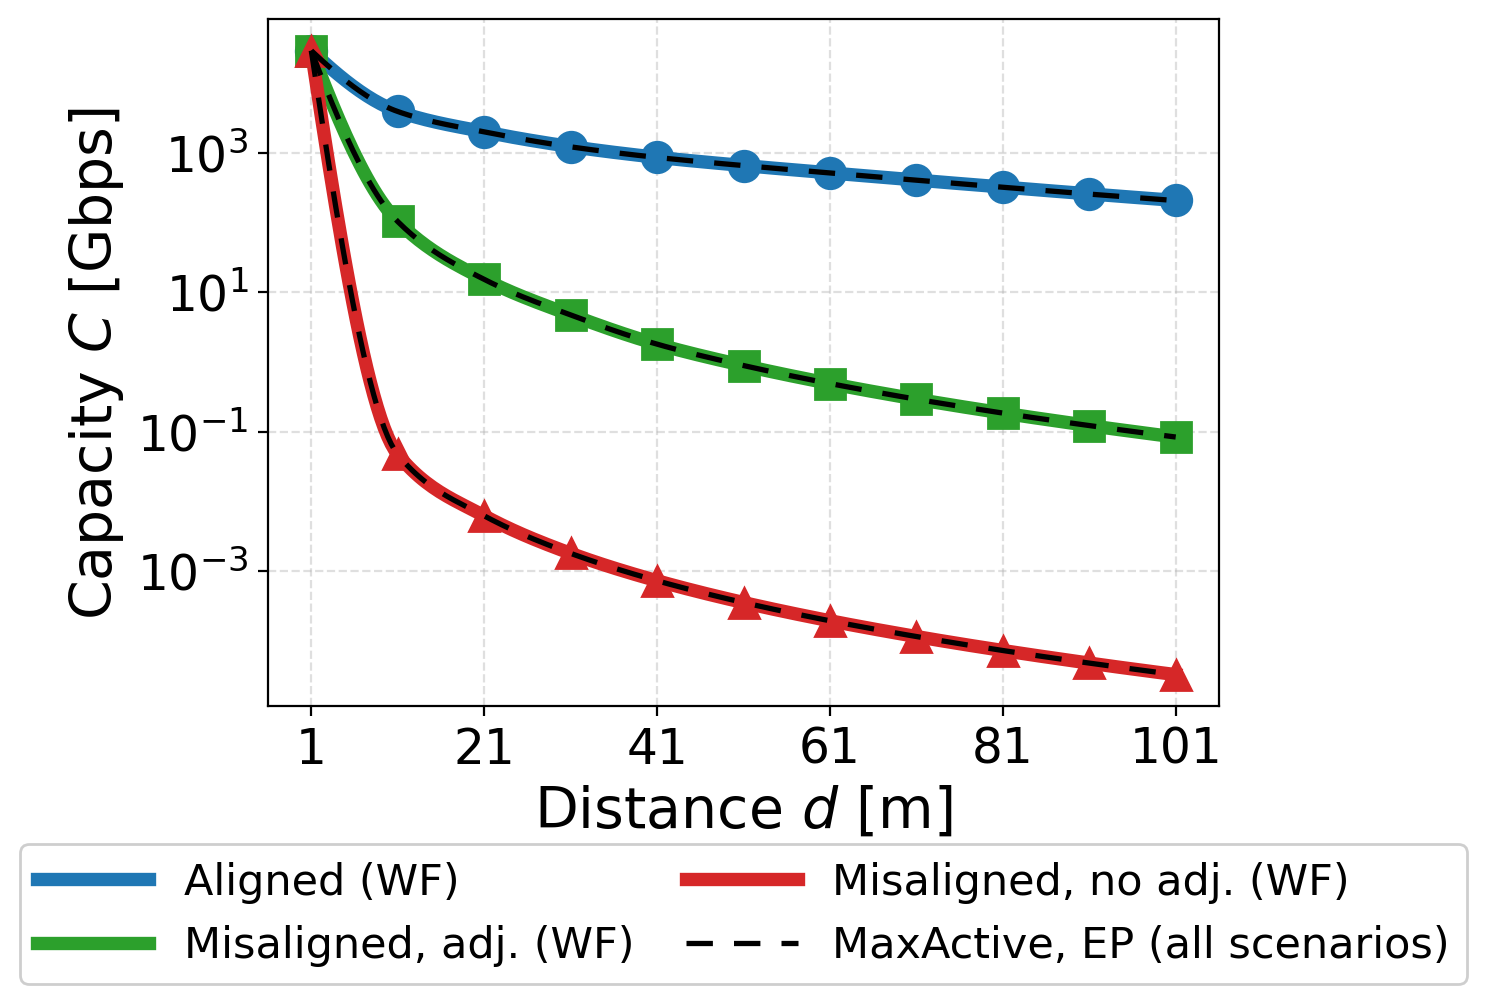
\includegraphics[width=\columnwidth]{maxactive_reference_single.png}
\caption{MaxActive reference capacity versus distance for the aligned link and for
diagonal mobility with and without beamwidth adjustment, under WF (thick, solid) and EP
(thin, dashed) allocation. The three scenarios occupy disjoint decades of the logarithmic
axis, spanning about nine orders of magnitude, and WF and EP nearly coincide throughout
(Section~\ref{sec:perf}-C). Curves are PCHIP-smoothed with markers at the true computed
distances.}
\label{fig:maxactive}
\end{figure}

\subsection{Dataset Construction and Scalability}
\label{sec:dataset}
For the supervised study we build one sample per scenario--distance pair. The main
dataset (aligned and the two diagonal scenarios) contains $33$ samples; the regression
target is $\log_{10}$ of the MaxActive capacity in Gbps, computed separately for WF and
EP. Each sample carries a $13$-dimensional physical feature vector: log-distance and its
square, normalized total gain and its square, normalized beamwidth, scenario
identifier, allocation flag, the mean and standard deviation of the per-sub-band
log-SNR, the mean and standard deviation of the log absorption-noise, the fraction of
valid sub-bands, and the normalized mean path loss. A separate $60$-sample dataset
($2\times19$ elevation points and $2\times11$ real-trace points) is constructed
identically for the additional mobility scenarios.

\emph{Why the dataset is small, and how it scales.} The sample count is set by the
reference model rather than by a sampling choice: the LBLRTM files resolve the
straight-line geometry at eleven ranges, and every extra sample costs a full physics
evaluation. Three properties make this regime workable rather than merely small. First,
the target is a deterministic, noiseless function of the features, so there is no label
noise to average out; $n$ controls only the resolution of the input space, not the
variance of the labels. Second, that space is low-dimensional and physically smooth, with
capacity varying monotonically in distance and misalignment, so a modest number of
well-spread points pins the surface down. Third, the evaluation protocol is matched to the
regime: nested cross-validation with $15$ outer folds (Section~\ref{sec:impl}), rather
than a single split, is what allows $18$ models to be ranked credibly on $33$ points.

Scaling up is straightforward but changes which model to prefer. Dataset generation is
embarrassingly parallel and linear in the number of operating points, at roughly
\PLMASTEP{} per sample, so a denser range grid, more beamwidths, additional carrier
configurations, or a swarm of links would push $n$ from tens to $10^4$--$10^6$ at a cost
of CPU-hours rather than new modeling. At that scale the $O(n^3)$ training and $O(n^2)$
memory of the Gaussian process become binding and the recommendation shifts to the tree
ensembles (Section~\ref{sec:complexity}). More data would also relax the main
generalization caveat: the present models are validated as \emph{interpolators} within the
envelope of geometries they were trained on, with no claim of extrapolation beyond it.
Since the reference model generates that data on demand, closing this gap is a matter of
compute rather than of method.

\section{Implementation}
\label{sec:impl}
The physical layer is reproduced in Python from the reference MATLAB model: the LBLRTM
transmittance is rescaled to the exact range (Beer--Lambert), and power allocation and
selection are solved in an outer loop (WF or EP, then MaxActive) that iterates until
the active set is stable; for the adjustment scenarios an inner search optimizes the
beamwidth per step. The elevation and real trajectories are ports of the MATLAB
hemisphere generator and acceleration integrator.

Because $33$ (or $60$) samples cannot support a single train/test split for ranking $18$
models, the reported metrics use \emph{nested} cross-validation. An outer repeated
$k$-fold loop ($5$ folds $\times\,3$ repeats $=15$ folds) estimates generalization, while
an inner $3$-fold grid search tunes hyper-parameters on the outer training partition only.
Feature standardization sits inside the pipeline, so it is fit on training folds alone and
leakage is eliminated. Grid search covers regularization strength for the
linear models, kernel width and penalty for SVR and kernel ridge, and depth and number of
estimators for the ensembles; the Gaussian process tunes its kernel internally by
marginal-likelihood maximization. Alongside RMSE and $R^2$ on the log target we report a
robust \emph{median relative error} in linear Gbps, which avoids the pathological
inflation of the mean absolute percentage error at the very small far-distance
capacities. Only the curves \emph{plotted} in the figures are evaluated at the ceiling
\eqref{eq:clip}, each model there being refit on all data (the estimator one would
deploy); every quantitative metric derives from raw, unclipped out-of-fold predictions,
keeping the generalization estimate independent of the clip.

The D3QN operates on individual SNR-ranked channels (top $N=500$, a $1000$-dimensional
state) at the same granularity as MaxActive-EP, with one lightweight bandit per
(distance, gain) context; the dueling network maps $1000\!\to\!16\!\to\!8$ to value and
advantage heads over $600$ actions, trained for $20$ epochs of $80$ $\epsilon$-greedy
actions (Adam, learning rate $10^{-3}$, weight decay $10^{-4}$).

\section{Performance Analysis}
\label{sec:perf}

\subsection{Regressors versus MaxActive}
Table~\ref{tab:cv} reports the nested cross-validated metrics for the EP target, sorted
best to worst by RMSE. The WF target was cross-validated identically; the two agree to
within $0.055$ RMSE for every one of the eighteen models, and to within $0.02$ for all but
the single decision tree, as the near-equality of the WF and EP capacities
(Table~\ref{tab:maxactive}) implies, so only the EP column is tabulated. Three findings
stand out. \emph{The smooth non-parametric and
kernel models win:} the Gaussian process is best by a wide margin ($R^2=0.99$, median
relative error $\approx1.9\%$), followed by ExtraTrees, SVR-RBF, MLP, and $k$-NN --- they
assume the smoothness the physical capacity curve actually exhibits, so they interpolate
MaxActive closely and generalize across folds. \emph{Regularized linear models are stable
but biased:} Ridge, Lasso, ElasticNet, and BayesianRidge hold $R^2\approx0.97$ with small
variance, yet their $\approx45\%$ median relative error reveals a systematic offset,
since a model affine in the features cannot capture the curvature of a capacity decaying
over nine decades. \emph{Cross-validation exposes failures a single split hides:} Huber
attains the best single-split accuracy but collapses to $R^2=0.93\pm0.10$ under CV, and
ordinary least squares is worse still ($R^2=-7.98\pm31$), dominated by unlucky folds;
with single decision trees and gradient boosting these are the failing methods. On $33$
points a single split is not trustworthy; the nested-CV mean$\,\pm\,$std is.

The last two columns of Table~\ref{tab:cv} quantify how far the \emph{raw} predictions
exceed the reference ceiling --- what the display clip of \eqref{eq:clip} conceals, and
equivalently the error a deployed surrogate would actually commit, having no ceiling to
clip against. Nearly every regressor crosses the bound somewhere, so violation magnitude
is a first-class selection criterion rather than a cosmetic detail. The piecewise-constant
single tree and plain gradient boosting overshoot by thousands of percent because they
cannot extrapolate the wide dynamic range, and a link budget dimensioned on such a
prediction would be badly optimistic. GaussProc and ExtraTrees, by contrast, stay within a
few percent, and the D3QN never violates the bound at all. Per-scenario, the
misaligned-without-adjustment case (the worst-SNR regime) is hardest for most models,
while GaussProc, SVR-RBF, kernel ridge, and $k$-NN stay within about $6\%$ across all
three main scenarios, marking them as the robust choices.

\begin{table}[!tbp]
\centering
\caption{Nested Cross-Validated Accuracy and Physical-Ceiling Violations
(EP Target, Ranked Best to Worst)}
\label{tab:cv}
\setlength{\tabcolsep}{2.5pt}
\scriptsize
\begin{tabular}{@{}l c c c c r@{}}
\toprule
& \multicolumn{3}{c}{Generalization (nested CV)} & \multicolumn{2}{c}{Ceiling viol.}\\
\cmidrule(lr){2-4}\cmidrule(lr){5-6}
Model & RMSE$\,\pm\,$std & $R^2$ & Med.\ rel. & pts. & max\\
\midrule
GaussProc           & $0.100\pm0.23$ & $0.991$  & $1.9\%$      & $19$       & $2.7\%$\\
ExtraTrees          & $0.237\pm0.18$ & $0.986$  & $12.1\%$     & $1$        & $3.7\%$\\
SVR-RBF             & $0.253\pm0.22$ & $0.982$  & $7.8\%$      & $18$       & $318\%$\\
MLP                 & $0.254\pm0.21$ & $0.980$  & $21.1\%$     & $20$       & $226\%$\\
BayesianRidge       & $0.331\pm0.14$ & $0.976$  & $42.5\%$     & $17$       & $322\%$\\
$k$-NN              & $0.338\pm0.29$ & $0.959$  & $9.0\%$      & $11$       & $111\%$\\
XGBoost             & $0.342\pm0.16$ & $0.970$  & $36.9\%$     & $14$       & $38\%$\\
KernelRidge         & $0.356\pm0.33$ & $0.962$  & $16.0\%$     & $17$       & $223\%$\\
Lasso/ENet/Ridge    & $0.36$--$0.37$ & $0.97$   & $45$--$49\%$ & $17$--$19$ & $232$--$261\%$\\
GradBoost           & $0.412\pm0.21$ & $0.957$  & $38.4\%$     & $16$       & $2993\%$\\
RF/Bag./AdaBoost    & $0.44$--$0.45$ & $0.96$   & $49$--$62\%$ & $9$--$11$  & $97$--$246\%$\\
Huber               & $0.504\pm0.37$ & $0.930$  & $48.4\%$     & $17$       & $1102\%$\\
DecisionTree        & $0.561\pm0.32$ & $0.931$  & $48.0\%$     & $3$        & $3698\%$\\
LinearReg           & $3.281\pm8.78$ & $-7.98$  & $55.8\%$     & $15$       & $405\%$\\
\midrule
D3QN (policy)       & ---            & ---      & $\sim\!0\%$  & $0$        & $0\%$\\
\bottomrule
\end{tabular}
\vspace{2pt}
\parbox{\columnwidth}{\scriptsize RMSE and $R^2$ are on the $\log_{10}$ target, the median
relative error in linear Gbps; all from \emph{raw, unclipped} out-of-fold predictions.
ENet $=$ ElasticNet, RF $=$ RandomForest, Bag.\ $=$ Bagging. ``pts.'' counts, out of $33$,
the points where the prediction exceeds the reference and ``max'' the largest such excess
--- what \eqref{eq:clip} conceals.}
\end{table}

Table~\ref{tab:perscen} breaks the out-of-fold median relative error down by scenario
for the strongest models, confirming that the smooth and kernel models remain accurate
even in the worst-SNR (misaligned, no adjustment) regime, whereas the tree ensembles
degrade there. This per-scenario stability, not merely a low aggregate error, is what
qualifies a model as a robust surrogate.

\begin{table}[!tbp]
\centering
\caption{Per-Scenario Median Relative Error (EP, Out-of-Fold)}
\label{tab:perscen}
\setlength{\tabcolsep}{6pt}
\footnotesize
\begin{tabular}{l c c c}
\toprule
Model & Aligned & Diag.\ no adj. & Diag.\ adj.\\
\midrule
GaussProc    & $2.0\%$ & $1.9\%$  & $0.8\%$\\
SVR-RBF      & $2.6\%$ & $5.3\%$  & $6.9\%$\\
KernelRidge  & $4.9\%$ & $6.0\%$  & $5.3\%$\\
$k$-NN       & $1.2\%$ & $20.1\%$ & $0.7\%$\\
ExtraTrees   & $2.7\%$ & $12.2\%$ & $24.6\%$\\
\bottomrule
\end{tabular}
\end{table}

\subsection{Mobility Scenarios and D3QN}
Extending the benchmark to the elevation and real-trace mobility patterns,
Fig.~\ref{fig:mlmob} overlays the ML predictions and the D3QN policy on the MaxActive
curves. Fitting on all data, the strongest models reproduce
these curves closely: XGBoost, GradBoost, and GaussProc reach median relative errors of
$0.07\%$, $0.7\%$, and $2.8\%$ over the elevation and real scenarios (Huber, $4.4\%$, is
next). Note that this is an in-sample fit, so it flatters models such as GradBoost that
fail under cross-validation --- which is precisely why Table~\ref{tab:cv}, not this fit,
is the basis for the ranking. Otherwise the family ordering of Table~\ref{tab:cv} is
visible: the smooth and kernel models hug the reference while the single tree and plain
linear model lag.
The D3QN, trained as a single-step contextual bandit at every trajectory point
(Section~\ref{sec:background}-C), reproduces the MaxActive EP capacity essentially
exactly on \emph{all seven} scenario variants: the mean capacity ratio is $99.9\%$ for
the aligned case and $100.0\%$ for each of the six misaligned cases --- diagonal,
elevation, and real-trace mobility, with and without beamwidth adjustment. The worst
single operating point over all $93$ evaluated geometries ($33$ in the main study plus
$60$ mobility points) still reaches $99.7\%$ of the reference, and no point exceeds it. Two points should
be read together. A learned policy operating at the same individual-channel granularity
as MaxActive-EP, driven by the capacity reward, recovers the reference selection rather
than merely a capacity estimate, and does so robustly under elevation and real-trace
mobility. But the result is bounded by construction: the policy searches the same
SNR-ordered prefixes MaxActive does, so $100\%$ means \emph{it found the same prefix},
not that it improved on the reference or solved a harder problem.

\begin{figure*}[!tp]
\centering
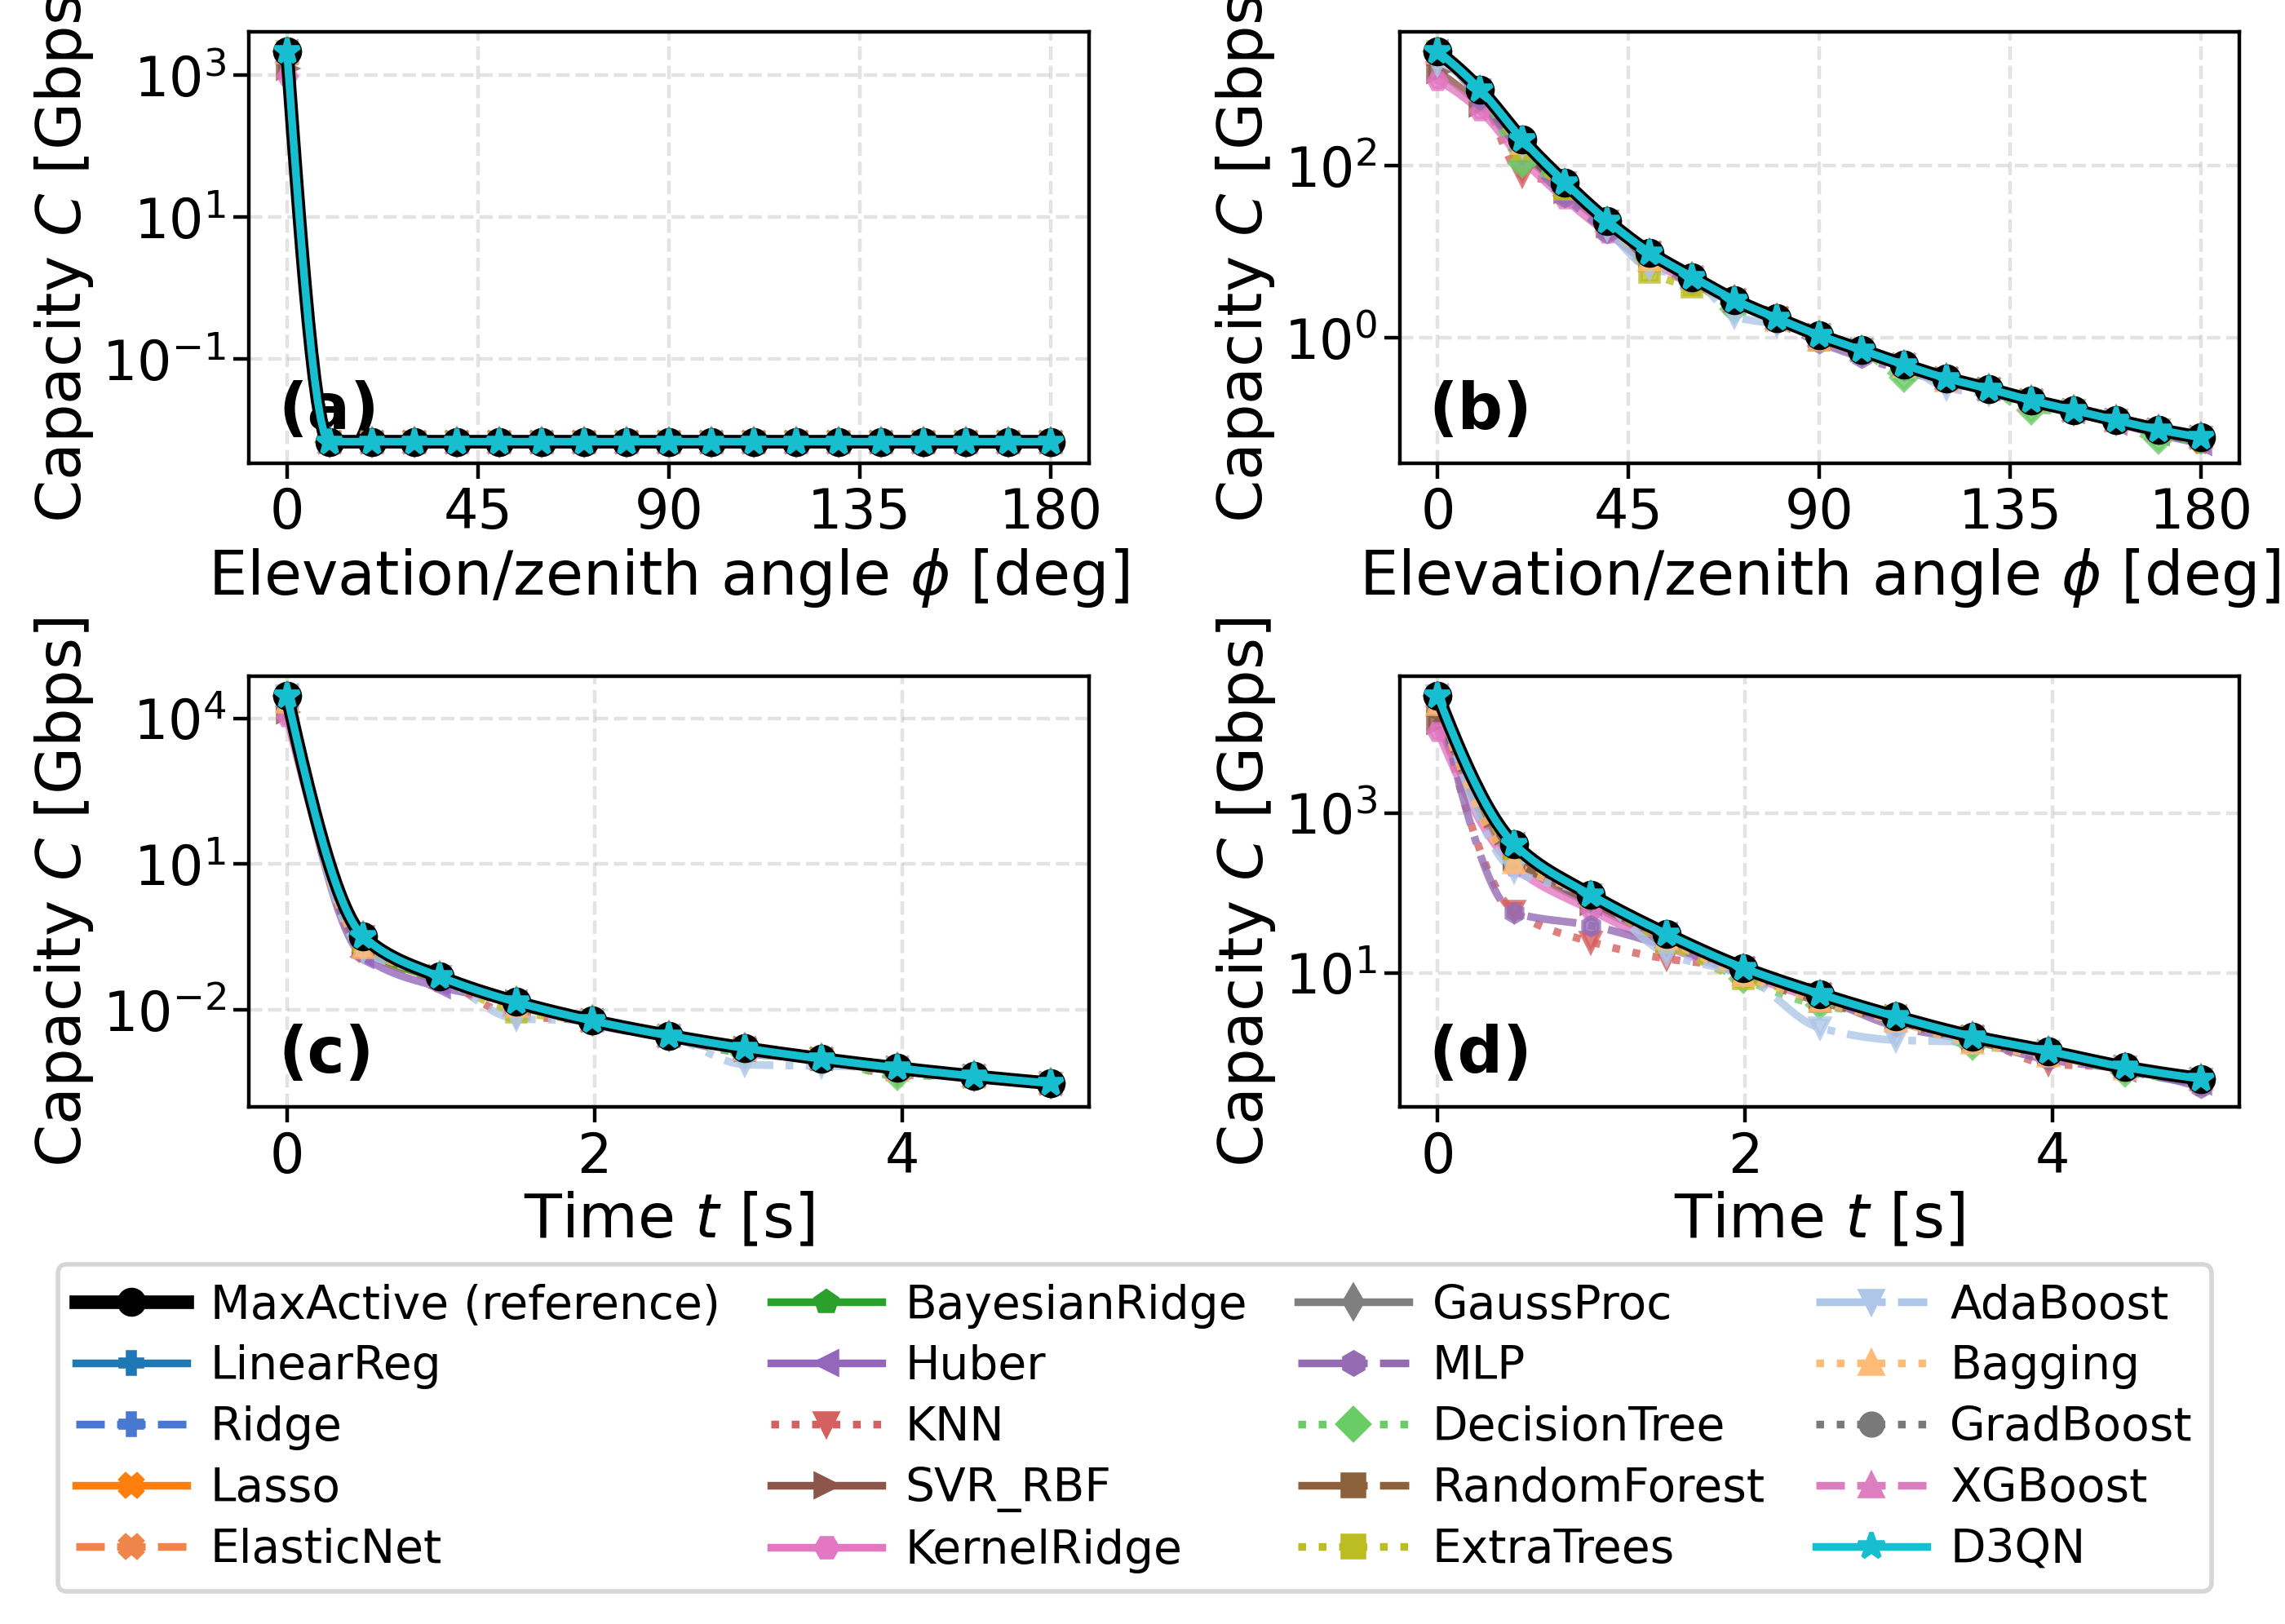
\includegraphics[width=0.92\textwidth]{ml_mobility_comparison.png}
\caption{All eighteen regressors and the D3QN versus MaxActive on the two additional
mobility patterns, under EP allocation: elevation mobility (a) without and (b) with
beamwidth adjustment, and real windy-hover traces (c) without and (d) with adjustment.
Without adjustment the elevation capacity falls to a side-lobe plateau once $\phi$ leaves
the beam, whereas adjustment gives a gradual decline; in the real traces the diagonal
drift produces the collapse and the measured accelerations the residual jitter. The WF
panels are omitted because WF and EP coincide to within the line width
(Table~\ref{tab:maxactive}). Curves are evaluated at the ceiling for display and
PCHIP-smoothed; D3QN (cyan) lies on the MaxActive curve throughout.}
\label{fig:mlmob}
\end{figure*}

\subsection{Discussion and Limitations}
\label{sec:discussion}
Three observations round out the analysis. First, the WF and EP capacities are nearly
identical across all scenarios (Table~\ref{tab:maxactive}): at THz the selected channels
already have comparable, high SNR, so the water-filling gain over equal power is
marginal, which justifies benchmarking the equal-power D3QN against MaxActive-EP. Second,
the contrast between the value regressors and the D3QN is the most transferable finding of
this study. The regressors predict a number and can exceed the physical bound. The D3QN
predicts a selection, and the capacity it reports is the one its choice actually delivers,
so it cannot exceed the reference --- which is why it attains $100\%$ of MaxActive-EP with
no clip anywhere in the pipeline. Where a surrogate must be trusted without supervision,
learning the decision is the safer target than learning its value.

Third, the study has limitations that bound these claims. The datasets are small ($33$ and
$60$ points) and physically smooth, which favors smoothness-assuming models and restricts
the validated regime to interpolation within the trained envelope
(Section~\ref{sec:dataset}). The surrogates are validated against a reference that is
itself optimal only within its threshold-search family (Section~\ref{sec:background}-B),
so they inherit that scope rather than approximating a globally optimal selector. The
regressors predict the capacity value rather than the selection mask, so a deployment that
needs the mask must use the D3QN branch, and the D3QN is in turn realized as per-context
bandits rather than a single geometry-generalizing policy (Section~\ref{sec:d3qn}).
Finally, all timings in Section~\ref{sec:complexity} come from a laptop-class CPU, so
absolute latencies on an embedded airborne processor will be larger. The
platform-independent quantity is the \emph{ratio} between search and surrogate, since both
slow down together on weaker hardware.

\section{Complexity, Runtime, and Deployment}
\label{sec:complexity}

\subsection{Asymptotic Cost}
MaxActive has per-step cost $O(Q\,|\mathcal{F}|)$ and must be re-run whenever the geometry
changes; it needs no training but incurs this search at every time step. The supervised
surrogates move that cost offline: the entire nested-CV benchmark of $18$ models over both
targets completes in about $80$~s on a CPU, dominated by the grid searches, and fitting
the $18$ deployable models on the full dataset takes $0.9$~s; afterwards a prediction is a
single forward, kernel, or neighbor evaluation. Table~\ref{tab:complexity} summarizes the
asymptotic training and prediction complexity of representative families ($n$ samples,
$d$ features, $T$ trees, $W$ network weights, $n_{sv}$ support vectors) together with
their measured cost and cross-validated accuracy, and adds the MaxActive and D3QN
references for context.

\subsection{Measured Execution Time}
\label{sec:runtime}
Asymptotics alone do not establish a practical benefit, so every stage was measured on
identical channel states, on a single core of an Intel Core i7-13620H with the band
discretized into $|\mathcal{F}|=\PLNCH$ active channels per context; the measured columns
of Table~\ref{tab:complexity} average the eleven aligned contexts.

The reference costs \PLMASEL{} for the threshold sweep alone, \PLMASTEP{} for a complete
link update with power allocation iterated to convergence, and \PLMASTEPBW{} with the
beamwidth search included, i.e., $1.2\times$ the fixed-beam cost on the same geometries.
Against this, the surrogate path costs $1.26$~ms to turn the channel state into the $13$
features and $31$--$63$~$\mu$s to evaluate a linear, kernel, or Gaussian-process model:
\PLPREDUS{} end-to-end, a $95\times$ reduction in per-update decision cost. Where that
factor comes from is worth stating precisely. The model evaluation alone is
$2000$--$4000\times$ faster than the search, but feature extraction now dominates the
online path. The end-to-end gain therefore saturates near two orders of magnitude, and
\emph{feature extraction, not inference, is the target for further optimization}. The
tree ensembles are the exception at the other end: they need $5.5$--$19$~ms per prediction
because hundreds of estimators must each be traversed, cutting their advantage to
$6$--$19\times$ and making them a poor per-update choice at this dataset size despite
their accuracy. The D3QN is the fastest decision of all: its state is built from the SNR
ranking MaxActive computes anyway ($0.83$~ms, shared by both), after which a forward pass
and $\arg\max$ take $0.11$~ms --- three orders of magnitude below the search --- and it
returns the selection itself rather than a capacity estimate. Its cost is paid offline:
$0.38$~s per context, about $13$~s for the $33$ contexts of the main study.

\subsection{Memory Footprint and Airborne Deployment}
\label{sec:deploy}
For a drone, memory and predictability matter as much as speed. The deployable artifacts
are small: the regularized-linear models occupy $1.2$--$2.2$~KB, SVR-RBF $4.6$~KB, the
Gaussian process $17.9$~KB (its $33\times33$ kernel and training inputs), the MLP $70$~KB,
and the D3QN $21\,561$ parameters, i.e., $84$~KB in single precision. Every one of these
fits in the on-chip memory of a microcontroller-class flight companion, and all are far
below the LBLRTM tables the reference search itself must hold. Only the tree ensembles
are heavy --- XGBoost
$522$~KB and ExtraTrees $1.4$~MB --- which, together with their millisecond-scale
inference, rules them out here despite their accuracy. Three further properties favor
deployment. Inference cost is constant and data independent, a fixed number of
multiply-accumulates with no search, iteration, or early exit, so the decision has a hard
worst-case latency that a threshold sweep of state-dependent length cannot offer. All
training is offline, so the platform performs no gradient computation and needs no
floating-point accelerator. And the arithmetic compresses further: an $8$-bit D3QN would
occupy $21$~KB, and the linear surrogates reduce to a $13$-element dot product. The
recommendation is therefore the Gaussian process where accuracy dominates ($18$~KB,
$63$~$\mu$s) and the D3QN where the selection mask is needed ($84$~KB, $0.11$~ms), with
the tree ensembles reserved for offline or ground-station use.

\begin{table*}[!tp]
\centering
\caption{Asymptotic and Measured Cost versus Accuracy of Representative Models}
\label{tab:complexity}
\footnotesize
\setlength{\tabcolsep}{5pt}
\renewcommand{\arraystretch}{1.2}
\begin{tabular}{@{}l l l r r r c c@{}}
\toprule
& \multicolumn{2}{c}{Asymptotic cost} & \multicolumn{3}{c}{Measured (single core, $n=33$)} &
  \multicolumn{2}{c}{Nested-CV accuracy (EP)}\\
\cmidrule(lr){2-3}\cmidrule(lr){4-6}\cmidrule(lr){7-8}
Model (family) & Training & Prediction & Train [ms] & Predict [ms] & Memory [KB] & $R^2$ & Med.\ rel.\ err.\\
\midrule
Ridge / Lasso (linear)            & $O(nd^2)$              & $O(d)$                    & $1.0$        & $0.039$          & $1.2$          & $0.97$          & $45\%$\\
$k$-NN (instance-based)           & $O(1)$ (store)         & $O(nd)$                   & $0.7$        & $0.331$          & $7.6$          & $0.96$          & $9\%$\\
DecisionTree (tree)               & $O(nd\log n)$          & $O(\text{depth})$         & $0.6$        & $0.043$          & $5.3$          & $0.93$          & $48\%$\\
XGBoost / ExtraTrees (ensemble)   & $O(T\,nd\log n)$       & $O(T\,\text{depth})$      & $175$--$191$ & $0.82$--$19.5$   & $522$--$1362$  & $0.97$--$0.99$  & $12$--$37\%$\\
MLP (neural)                      & $O(\text{it}\cdot nW)$ & $O(W)$                    & $82$         & $0.049$          & $70$           & $0.98$          & $21\%$\\
SVR-RBF (kernel)                  & $O(n^2\!-\!n^3)$       & $O(n_{sv}d)$              & $1.3$        & $0.055$          & $4.6$          & $0.98$          & $8\%$\\
\textbf{GaussProc} (kernel/prob.) & $O(n^3)$, mem $O(n^2)$ & $O(n)$ mean               & $22$         & $\mathbf{0.063}$ & $\mathbf{17.9}$ & $\mathbf{0.99}$ & $\mathbf{1.9\%}$\\
\midrule
MaxActive (reference)             & --- (online search)    & $O(Q|\mathcal{F}|)$ / step & ---         & $\mathbf{125.6}$ & ---            & reference       & ---\\
D3QN (policy)                     & $O(E\cdot A)$ / context & $O(\text{forward pass})$  & $384$/ctx.  & $0.11$           & $84$           & $\approx$ ref.  & $\sim\!0\%$\\
\bottomrule
\end{tabular}
\vspace{2pt}
\parbox{0.97\textwidth}{\footnotesize Prediction times are per operating point and exclude
the $1.26$~ms feature extraction shared by all regressors (Section~\ref{sec:runtime}); the
MaxActive row is the threshold sweep alone, on the same channel states. Memory is the
serialized model size; for the D3QN it is $21\,561$ parameters in single precision.}
\end{table*}

\subsection{Accuracy versus Complexity, and Convergence}
\emph{Best models but higher complexity.} A clear accuracy-versus-complexity trade-off
emerges, and it is the central practical conclusion of this study. The most accurate
surrogate, the Gaussian process, is the most expensive to train ($O(n^3)$ time, $O(n^2)$
memory, prediction requiring the full training kernel); the next best, SVR-RBF and kernel
ridge, are likewise kernel-based at $O(n^2\!-\!n^3)$; and the cheapest models
($O(nd^2)$ training, $O(d)$ prediction) are systematically biased ($\approx45\%$ median
error). The accuracy ranking of Table~\ref{tab:cv} therefore roughly tracks the cost
ranking of Table~\ref{tab:complexity}: the last few percent of accuracy is bought at a
super-linear price in the number of samples.

Two regimes invert the recommendation, however. At the present scale ($n\le60$) the
asymptotic penalty is invisible in wall-clock terms: the Gaussian process trains in
$22$~ms and predicts in $63$~$\mu$s, cheaper at inference than $k$-NN or any ensemble. The
most accurate model can therefore simply be chosen, and GaussProc is the recommended
surrogate here. What costs time at this scale is the number of estimators rather than the
asymptotic class, which is why the tree ensembles are the slowest predictors in the table.
As $n$ grows toward the $10^4$--$10^6$ samples of Section~\ref{sec:dataset}, the cubic
training and quadratic memory of the kernel methods become prohibitive while the ensembles
amortize their per-tree overhead, and the sweet spot shifts to XGBoost and ExtraTrees. The
rule is: kernel methods while the dataset is small, tree ensembles once it is not.

Convergence is not a limiting factor for either learned method. The D3QN converges for the
structural reason given in Section~\ref{sec:background}-C --- each context is a single-step
bandit with a deterministic reward, so there is no bootstrapping variance and no
credit-assignment horizon --- and $20$ epochs of $80$ actions suffice to reach the
reference capacity. The coupled WF/MaxActive loop inside the reference itself converges in
a handful of iterations, since each MaxActive step can only refine an SNR-ordered prefix.

\section{Conclusion}
Machine-learning models can replace the online MaxActive search in mobile THz drone
links, and the experiments identify which kinds, and why. Three findings carry beyond
this system. First, the inductive bias that matters here is smoothness: the physical
capacity surface is smooth and wide-ranging, so kernel and Gaussian-process models track
the reference closely while piecewise-constant learners cannot extrapolate it and
overshoot the physical bound by orders of magnitude. Second, on datasets this small the
evaluation protocol decides the ranking --- a single split reorders the models and hides
overfitting, so nested cross-validation is not a refinement but a requirement. Third, and
most transferable, learning the \emph{decision} is safer than learning its \emph{value}:
a policy that selects channels and reports the capacity its choice actually delivers
inherits the reference's feasibility guarantee, whereas a value regressor can predict a
rate the link cannot support.

The practical implication is that the surrogate is limited by feature extraction rather
than by inference, and that its memory footprint suits a microcontroller-class flight
computer. The accuracy-optimal model can therefore be deployed as is; only as the dataset
grows by orders of magnitude does the super-linear cost of the kernel methods force a
switch to tree ensembles. Future work will replace the per-context bandits with a single
geometry-generalizing policy, predict the selection mask rather than the capacity value,
and extend the dataset into the regime where that trade-off binds.

\begin{thebibliography}{10}
\bibitem{jornet}
J.~M. Jornet and I.~F. Akyildiz,
``Channel modeling and capacity analysis for electromagnetic wireless nanonetworks in
the terahertz band,''
\emph{IEEE Trans. Wireless Commun.}, vol.~10, no.~10, pp.~3211--3221, Oct. 2011.

\bibitem{mnih}
V.~Mnih \emph{et al.},
``Human-level control through deep reinforcement learning,''
\emph{Nature}, vol.~518, no.~7540, pp.~529--533, 2015.

\bibitem{vanhasselt}
H.~van Hasselt, A.~Guez, and D.~Silver,
``Deep reinforcement learning with double $Q$-learning,''
in \emph{Proc. AAAI Conf. Artif. Intell.}, 2016, pp.~2094--2100.

\bibitem{wang}
Z.~Wang, T.~Schaul, M.~Hessel, H.~van Hasselt, M.~Lanctot, and N.~de Freitas,
``Dueling network architectures for deep reinforcement learning,''
in \emph{Proc. Int. Conf. Mach. Learn. (ICML)}, 2016, pp.~1995--2003.

\bibitem{rasmussen}
C.~E. Rasmussen and C.~K.~I. Williams,
\emph{Gaussian Processes for Machine Learning}.
Cambridge, MA, USA: MIT Press, 2006.

\bibitem{xgboost}
T.~Chen and C.~Guestrin,
``XGBoost: A scalable tree boosting system,''
in \emph{Proc. ACM SIGKDD Int. Conf. Knowl. Discovery Data Mining}, 2016,
pp.~785--794.

\bibitem{sklearn}
F.~Pedregosa \emph{et al.},
``Scikit-learn: Machine learning in Python,''
\emph{J. Mach. Learn. Res.}, vol.~12, pp.~2825--2830, 2011.

\bibitem{shannon}
C.~E. Shannon,
``A mathematical theory of communication,''
\emph{Bell Syst. Tech. J.}, vol.~27, pp.~379--423, 1948.
\end{thebibliography}

\end{document}
